\documentclass[12pt]{report}
\usepackage{graphicx}
\usepackage{titling}
\usepackage{fancyhdr}
\usepackage[latin1]{inputenc}
\usepackage{enumerate}
\usepackage{float}
\usepackage{latexsym}
\usepackage{amssymb}
\usepackage{amsthm}
\usepackage{amsfonts}
\usepackage{amsmath}
\usepackage[labelfont=bf]{caption}
\usepackage[usenames,dvipsnames,svgnames,table]{xcolor}
\usepackage{listings}
\parindent=0pt
\frenchspacing

\pagestyle{fancy}

\newcommand{\pctlrepeat}[1]{{\buildrel{#1}\over\curvearrowleft}}

\fancyhead[L]{\slshape\footnotesize December 3, 2013\\\textsc{02246 Model Checking}}
\fancyhead[R]{\slshape\footnotesize \textsc{Andreas Kjeldsen (s092638)}\\\textsc{Morten Eskesen (s133304)}}
\fancyfoot[C]{\thepage}

\lstdefinestyle{logoutput}{
	backgroundcolor=\color[RGB]{248,248,248},
	tabsize=1,
	captionpos=b
  	belowcaptionskip=1\baselineskip,
  	breaklines=true,
  	frame=single,
	language={},
  	basicstyle=\footnotesize\ttfamily\color{Black}
}

\lstdefinestyle{prismmodel}{
	tabsize=1,
	captionpos=b,
  	belowcaptionskip=1\baselineskip,
  	breaklines=true,
  	frame=single,
	frameround=tttt,
  	language={},
  	numbers=left,
  	numbersep=5pt,
  	numberstyle=\tiny\ttfamily\color{Black},
  	basicstyle=\footnotesize\ttfamily\color{Black},
  	keywordstyle=\bfseries\color{Black},
	morekeywords={module, endmodule, label, init, mdp }, 
	otherkeywords={=, :, [, ], |},
	identifierstyle={\color{red}\let\textcolor\textcolordummy},
	morestring=[b][\color{red}\bfseries]",
	commentstyle=\color{Green},
	moredelim=[s][\color{DarkOrchid}\ttfamily]{[}{]},
	literate=%
		*{0}{{{\color{blue}0}}}1
	    {1}{{{\color{blue}1}}}1
	    {2}{{{\color{blue}2}}}1
	    {3}{{{\color{blue}3}}}1
	    {4}{{{\color{blue}4}}}1
	    {5}{{{\color{blue}5}}}1
	    {6}{{{\color{blue}6}}}1
	    {7}{{{\color{blue}7}}}1
	    {8}{{{\color{blue}8}}}1
	    {9}{{{\color{blue}9}}}1
}

\newcommand{\tab}{\hspace*{2em}}
\newcommand{\HRule}{\rule{\linewidth}{0.5mm}}

\begin{document}

\begin{titlepage}
\begin{center}


\includegraphics[scale=2.0]{../GFX/dtu_logo.pdf}\\[1cm]

\textsc{\LARGE Technical University of Denmark}\\[1.5cm]

\textsc{\Large 02246 Model Checking}\\[0.5cm]


% Title
\HRule \\[0.4cm]
{\huge \bfseries Mandatory Assignment\\Part 2: Stochastic Modelling and Verification in Discrete Time}\\[0.1cm]
\HRule \\[1.5cm]

% Author and supervisor
\large
\emph{Authors:}
\\[10pt]
Andreas Hallberg \textsc{Kjeldsen}\\
\emph{s092638@student.dtu.dk}
\\[10pt]
Morten Chabert \textsc{Eskesen}\\
\emph{s133304@student.dtu.dk}

\vfill

% Bottom of the page
{\large December 3, 2013}

\end{center}
\end{titlepage}

\chapter*{Introductory notes}
This report has been written by the both of us. All parts have been worked on together and therefore our responsibility for each assignment is equal.
\chapter*{Part A: Introductory Problems}
\section*{A1) Practical Problems}

\subsection*{A1.1}
In this problem we will ad probabilities to the FCFS scheduler from the previous assignment, so that we construct a discrete time Markov chain.

\subsubsection*{A1.1a)}
Currently in the FCFS scheduler there are sources of non-determinism. Some of the sources are the create commands in $client_1$ and $client_2$ because there are 5 different create commands with the same guard only the update distinguishes the commands. These sources are due to local non-determinism between the commands in the modules. The other source of non-determinism is due to concurrent execution of the modules in FCFS. The shifting command in the Scheduler module is a result of non-determinism because it can happen independently of what the other modules are doing.

\subsubsection*{A1.1b)}
In order to resolve the local non-determinism we have to modify the modules to include probabilistic commands. Since the distribution of the probabilities should be uniform the new create command will look like the following:
\begin{lstlisting}[style=prismmodel]
[create1] state1=0 -> 0.2 :(state1'=1) & (task1'=1) +
                      0.2 :(state1'=1) & (task1'=2) +
                      0.2 :(state1'=1) & (task1'=3) +
                      0.2 :(state1'=1) & (task1'=4) + 
                      0.2 :(state1'=1) & (task1'=5);
\end{lstlisting}

\subsubsection*{A1.1c)}
The FCFS file has been changed to have the extension .pm and the first line of the model is 'dtmc' which tells PRISM that the file describes a Discrete Time Markov Chain. Building the model causes no errors and tells us that we now have 83 reachable states in the model. Which was the same as before because PRISM resolves the local non-determinism by using a uniform distribution. If there are 5 possibilities it will choose each with probability $\frac{1}{5}$.

\subsubsection*{A1.1d)}
As explained earlier the shifting command in the Scheduler module causes some non-determinism. This non-determinism we have due to the concurrent execution of the modules is still there. If there were commands in the other commands in the modules that could happen independently of what the Scheduler module was doing all of these commands would happen with equal probability. Since there are no other commands specified that way the command in the Scheduler module happens with probability 1 when possible. PRISM enforces this.

\subsubsection*{A1.1e)}
In order to make sure that a job will almost certainly complete we specify the following PRISM properties - one for each client.
\begin{center}
$(task_1 > 0) \Rightarrow P_{\geq 1}(F(task_1 = 0))$\\
$(task_2 > 0) \Rightarrow P_{\geq 1}(F(task_2 = 0))$
\end{center}
These properties have been verified by PRISM so we now know that a created job will almost certainly complete in this model.

\subsection*{A1.2}
This section is about using PRISM to compute numerical properties of the FCFS model.

\subsubsection*{A1.2a)}
If we calculate the steady state distribution of the model we can find the probability of having no jobs in the scheduler. We use PRISM to calculate the steady state distribution and it gives us the probability of being in each of the reachable states. Only one state has no jobs in the scheduler which is the initial:
\begin{center}
0:(0,0,0,0,0,0)=0.016145825133811565
\end{center}
The probability of having no jobs in the scheduler is therefore 0.0161.

\subsubsection*{A1.2b)}
We want to calculate the expected length of a job for $client_1$ by looking at the steady state probabilities. In order to do this computation manually we first have to sum the probabilities of the states where $client_1$ has a job of length $i$, $0 \leq i \leq 5$. These states are states 12-82.

\subsubsection*{A1.2c)}
We want to know what the probability of $client_1$ not having a job at time $t = 10$ so we calculate the transient distribution of the model at time $t = 10$. When we do this PRISM will output the probability for being in each state at this time and we sum the probabilities of being in states where $client_1$ does not have a job. States where $client_1$ does not have a job are states 0-11. We sum the probability of being in these states and get:
\begin{center}
Probability: 0.2574
\end{center}

\subsubsection*{A1.2d)}


\subsection*{A1.3}


\subsubsection*{A1.3a)}


\subsubsection*{A1.3b)}


\subsubsection*{A1.3c)}


\subsubsection*{A1.3d)}


\subsection*{A1.4}


\subsubsection*{A1.4a)}


\subsubsection*{A1.4b)}


\subsubsection*{A1.4c)}


\subsubsection*{A1.4d)}


\section*{A2) Theoretical Problems}
\begin{figure}[H]
	\begin{center}
		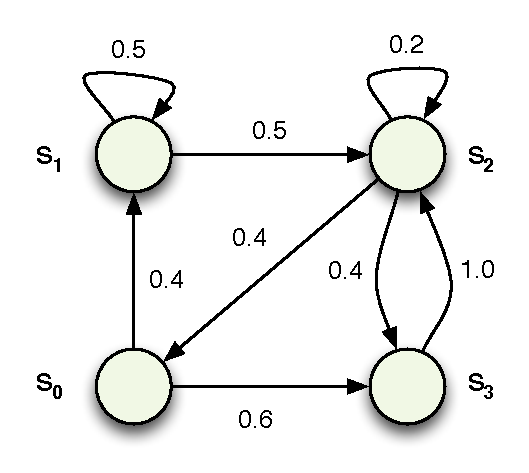
\includegraphics[scale=.85]{../GFX/ExerciseFigure1.pdf}
	\end{center}
	\caption{DTMC for questions A2.1 and A2.2}
	\label{fig:2a12}
\end{figure}

\subsection*{A2.1}
We have to consider the DTMC in Figure \ref{fig:2a12}, which is shown above and have initial state $s_0$.

\subsubsection*{A2.1a) Probability transition}
The initial distribution for the DTMC is as follows:
$$\iota_{init} = \left(1, 0, 0, 0\right)$$

The probability transition matrix for the DTMC is as follows:
$$\mathrm{\textbf{P}} = \left(
\begin{array}{c c c c}
	0 & 0.4 & 0 & 0.6\\
	0 & 0.5 & 0.5 & 0\\
	0.4 & 0 & 0.2 & 0.4\\
	0 & 0 & 1 & 0
\end{array}
\right)$$

\subsubsection*{A2.1b) Transient distribution}
The transient distribution, $\Theta$, up until the first three time steps is as follows:
\begin{center}
	\begin{tabular}{c c c c c c c c}
	& & & $s_0$ & $s_1$ & $s_2$ & $s_3$\\
	$\Theta_0$ & = & [ & 1.00 & 0.00 & 0.00 & 0.00 & ]\\
	$\Theta_1$ & = & [ & 0.00 & 0.40 & 0.00 & 0.60 & ]\\
	$\Theta_2$ & = & [ & 0.00 & 0.20 & 0.80 & 0.00 & ]\\
	$\Theta_3$ & = & [ & 0.32 & 0.10 & 0.26 & 0.32 & ]
	\end{tabular}
\end{center}

\subsubsection*{A2.1c) Steady state solution}
We have to calculate the steady state solution. First off, let's write down the equation matrix.
$$
	\left[
	\begin{matrix}
		P_1 & P_2 & P_3 & P_4
	\end{matrix}
	\right] \left[
	\begin{matrix}
		0 & 0.4 & 0 & 0.6\\
		0 & 0.5 & 0.5 & 0\\
		0.4 & 0 & 0.2 & 0.4\\
		0 & 0 & 1 & 0
	\end{matrix}
	\right] = \left[
	\begin{matrix}
		P_1 & P_2 & P_3 & P_4
	\end{matrix}
	\right]
$$
Now let's solve the equation.
\begin{description}
	\item[Step 1] Writing up the equations.
	$$\begin{array}{r c l c}
		P_1 & = & 0P_1 + 0P_2 + 0.4P_3 + 0P_4 & \Rightarrow\\
		P_1 & = & 0.4P_3\\
		\\
		P_2 & = & 0.4P_1 + 0.5P_2 + 0P_3 + 0P_3 & \Rightarrow\\
		P_2& = & 0.4P_1 + 0.5P_2\\
		\\
		P_3 & = & 0P_1 + 0.5P_2 + 0.2P_3 + P_4 & \Rightarrow\\
		P_3 & = & 0.5P_2 + 0.2P_3 + P_4\\
		\\
		P_4 & = & 0.6P_1 + 0P_2 + 0.4P_3 + 0P_4 & \Rightarrow\\
		P_4 & = & 0.6P_1 + 0.4P_3\\
		\\
		1 & = & P_1 + P_2 + P_3 + P_4
	\end{array}$$
	
	\item[Step 2] Reducing the equations.
	$$\begin{array}{r c l c}
		P_1 & = & 0.4P_3\\
		\\
		P_2 & = & 0.4P_1 + 0.5P_2 & \Rightarrow\\
		0.5P_2 & = & 0.4P_1 & \Rightarrow\\
		P_2 & = & 0.8P_1\\
		\\
		P_3 & = & 0.5P_2 + 0.2P_3 + P_4 & \Rightarrow\\
		0.8P_3 & = & 0.5P_2 + P_4 & \Rightarrow\\
		P_3 & = & 0.625P_2 + 1.25P_4\\
		\\
		P_4 & = & 0.6P_1 + 0.4P_3
	\end{array}$$
	
	\item[Step 3] Substituting $P_1$.
	$$\begin{array}{r c l c}
		P_2 & = & 0.8(0.4P_3) & \Rightarrow\\
		P_2 & = & 0.32P_3\\
		\\
		P_4 & = & 0.6(0.4P_3) + 0.4P_3 & \Rightarrow\\
		P_4 & = & 0.24P_3 + 0.4P_3 & \Rightarrow\\
		P_4 & = & 0.64P3\\
		\\
		1 & = & 0.4P_3 + P_2 + P_3 + P_4 & \Rightarrow\\
		1 & = & P_2 + 1.4P_3 + P_4
	\end{array}$$
	
	\item[Step 4] Substituting $P_2$.
	$$\begin{array}{r c l c}
		P_3 & = & 0.625(0.32P_3) + 1.25P_4 & \Rightarrow\\
		P_3 & = & 0.2P_3 + 1.25P_4 & \Rightarrow\\
		0.8P_3 & = & 1.25P_4 & \Rightarrow\\
		P_3 & = & 1.5625P_4\\
		\\
		1 & = & 0.32P_3 + 1.4P_3 + P_4 & \Rightarrow\\
		1 & = & 1.72P_3 + P_4
	\end{array}$$
	
	\item[Step 5] Calculating $P_3$.
	$$\begin{array}{r c l c}
		1 & = & 1.72P_3 + 0.64P_3 & \Rightarrow\\
		1 & = & 2.36P_4 & \Rightarrow\\
		P_3 & = & \frac{1}{2.36} & \Rightarrow\\
		P_3 & = & 0.42372881355 
	\end{array}$$
	
	\item[Step 5] Calculating $P_4$.
	$$\begin{array}{r c l c}
		1 & = & 1.72(1.5626P_4) + 1P_4 & \Rightarrow\\
		1 & = & 2.687672P_4 + 1P_4 & \Rightarrow\\
		1 & = & 3.687662P_4 & \Rightarrow\\
		P_4 & = & \frac{1}{3.687662} & \Rightarrow\\
		P_4 & = & 0.27117452738 
	\end{array}$$
	
	\item[Step 6] Calculating $P_1$.
	$$\begin{array}{r c l c}
		P_1 & = & 0.4P_3 & \Rightarrow\\
		P_1 & = & 0.4(0.42372881355) & \Rightarrow\\
		P_1 & = & 0.16949152542
	\end{array}$$
	
	\item[Step 7] Calculating $P_2$.
	$$\begin{array}{r c l c}
		P_2 & = & 0.8P_1 & \Rightarrow\\
		P_2 & = & 0.8(0.16949152542) & \Rightarrow\\
		P_2 & = & 0.13559322033
	\end{array}$$
\end{description}

So to sum up we have the following steady state probabilities for the DTMC:
$$\left[
	\begin{matrix}
		0.16949152542 & 0.13559322033 & 0.42372881355 & 0.27117452738
	\end{matrix}
\right]$$

\subsection*{A2.2}
The DTMC from Figure \ref{fig:2a12} encoded as a PRISM module:
\lstinputlisting[style=prismmodel,caption={PRISM module encoding the DTMC from Figure \ref{fig:2a12}.}]{../Code/A2.2.pm}

PRISM outputs the following transient distribution for the encoded DTMC:
\begin{lstlisting}[style=logoutput]
0:(0)=0.32000000000000006
1:(1)=0.1
2:(2)=0.26
3:(3)=0.32000000000000006
\end{lstlisting}
The above matches the calculated transient distribution from A2.1b.\\
\\
PRISM outputs the following steady state probabilities for the encoded DTMC:
\begin{lstlisting}[style=logoutput]
0:(0)=0.1694916167456058
1:(1)=0.1355931954330166
2:(2)=0.42372867450100926
3:(3)=0.2711865133203683
\end{lstlisting}
The above matches the calculated steady state solution from A2.1c.

\subsection*{A2.3}
\begin{figure}[H]
	\begin{center}
	\begin{tabular}{c c}
		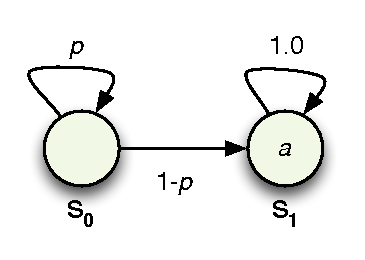
\includegraphics[scale=.85]{../GFX/ExerciseFigure2a.pdf} &
		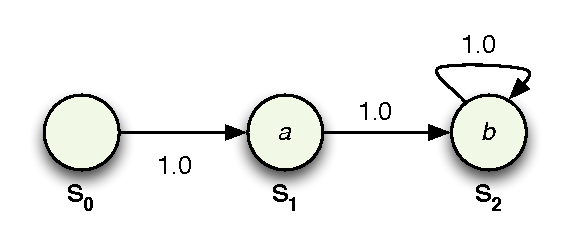
\includegraphics[scale=.85]{../GFX/ExerciseFigure2b.pdf}\\
		\textbf{\Large(a)} & \textbf{\Large(b)}
	\end{tabular}
	\end{center}
	\caption{DTMCs for question A2.3}
	\label{fig:2a3}
\end{figure}

We have to consider the DTMC in Figure \ref{fig:2a3}(a), which is shown above and have initial state $s_0$.

\subsubsection*{A2.3a) Values for $p$ which holds for $s_0 \models \mathbb{P}_{\geq \frac{1}{2}}(F^{\leq 2}\; a)$}
We have a maximum of two steps to reach $a$ with a probability of at least $\frac{1}{2}$. In other words we have to solve:
$$(1-p)^2 \geq \frac{1}{2} \quad | \quad 0 \leq p \leq 1$$

This gives:
$$0 \leq p \leq 0.292893$$

\subsubsection*{A2.3b) Expected number of time steps until $a$ holds in terms of $p$}
We have to calculate the \emph{Markov chain sojourn time}. We look at the probability of leaving the initial state $s_0$, thereby reaching $a$ for some amount of steps.

\begin{description}
	\item[Define $p_s$] The probability of staying in the same state, in this case $s_0$, is defined as:
	$$p_s = 1 - P(s_0, s_0)$$
	
	\item[Probability after one time step] The probability of staying in $s_0$ after one time step is:
	$$\mathrm{\textbf{Pr}}_{s_0}(N_{s_0}=1)=p_s$$
	
	\item[Probability after two time steps] The probability of staying in $s_0$ after two time steps is:
	$$\mathrm{\textbf{Pr}}_{s_0}(N_{s_0}=2)=(1-p_s) \cdot p_s$$
	
	\item[Probability after $n$ time steps] The probability of staying in $s_0$ after $n$ time steps is:
	$$\mathrm{\textbf{Pr}}_{s_0}(N_{s_0}=n)=(1-p_s)^{(n-1)} \cdot p_s$$
	
	\item[Rewriting] The probability of staying in $s_0$ after $n$ times steps can also be written as:
	$$\mathrm{\textbf{Pr}}_{s_0}(N_{s_0} \leq n) = \sum_{i=1}^{n} \mathrm{\textbf{Pr}}_{s_0}(N_{s_0} = i)  = 1 - (1-p_s)^n$$
	
	\item[Expected number of time steps spend in state $s_0$] Can be calculated using the formula below:
	$$\begin{array}{r c l}
	\mathrm{E}[N_{s_0}] & = & \sum_{i=1}^{n} \mathrm{\textbf{Pr}}_{s_0}(N_{s_0} = i)\cdot i\\[0.15cm]
	& = & \sum_{n=1}^{\infty} \mathrm{\textbf{Pr}}_{s_0}(N_{s_0} \geq n)\\[0.15cm]
	& = & \sum_{n=1}^{\infty} (1-p_s)^{n-1}\\[0.15cm]
	& = & \frac{1}{p_s}
	\end{array}$$
	
	\item[Replacing $p_s$] We have to state the expected number of time steps in terms of $p$, therefore we start by replacing $p_s$:
	$$\mathrm{E}[N_{s_0}] = \frac{1}{1 - P(s_0,s_0)}$$
	We then replace $P(s_0,s_0)$:
	$$\mathrm{E}[N_{s_0}] = \frac{1}{1 - p}$$
\end{description}

%sum((1-x)^(n-1)*x, n, 1, y) = 1-(1-x)^y

\subsubsection*{A2.3c) DTMC modification}
We have to modify Figure \ref{fig:2a3}(b), without increasing the number of states, so that the following holds:
$$s_0 \models \mathbb{P}_{\geq \frac{1}{2}}(F^{=5}\; a)$$
$$s_1 \models \mathbb{P}_{\geq \frac{1}{2}}(F^{=10}\; b)$$

\begin{description}
	\item[Reaching $s_1$ from $s_0$] To do this in five time steps we have to calculate the probability of $s_0$ going to $s_0$, while ensuring that on average 5 time time steps will be enough to reach $s_1$. We calculate it the following way:
	$$5 = \frac{1}{1-p} \Rightarrow \ldots \Rightarrow p = \frac{4}{5}$$
	So to ensure that on average 5 time steps will be required to go from $s_0$ to $s_1$ we must add the following to the DTMC:
	$$s_0 \xrightarrow{0.8} s_0$$
	
	\item[Reaching $s_2$ from $s_1$] To do this in 10 time steps we have to calculate the probability of $s_1$ going to $s_1$, while ensuring that on average 10 time steps will be enough to reach $s_2$. We calculate it the following way:
	$$10 = \frac{1}{1-p} \Rightarrow \ldots \Rightarrow p = \frac{9}{10}$$
	So to ensure that on average 10 time steps will be required to go from $s_1$ to $s_2$ we must add the following to the DTMC:
	$$s_1 \xrightarrow{0.9} s_1$$
	
	\item[The modified DTMC] Below is the modified DTMC:
	\begin{figure}[H]
		\begin{center}
		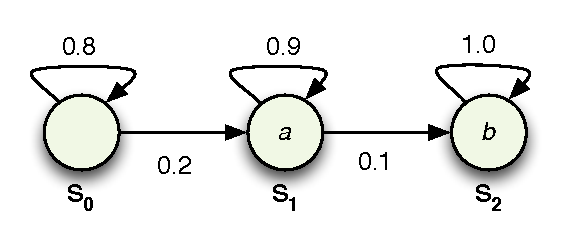
\includegraphics[scale=.85]{../GFX/Answer-A2-3c.pdf}
		\end{center}
		\caption{Modified version of the DTMC from Figure \ref{fig:2a3}.}
	\end{figure}
\end{description}

\subsection*{A2.4}
\begin{figure}[H]
	\begin{center}
		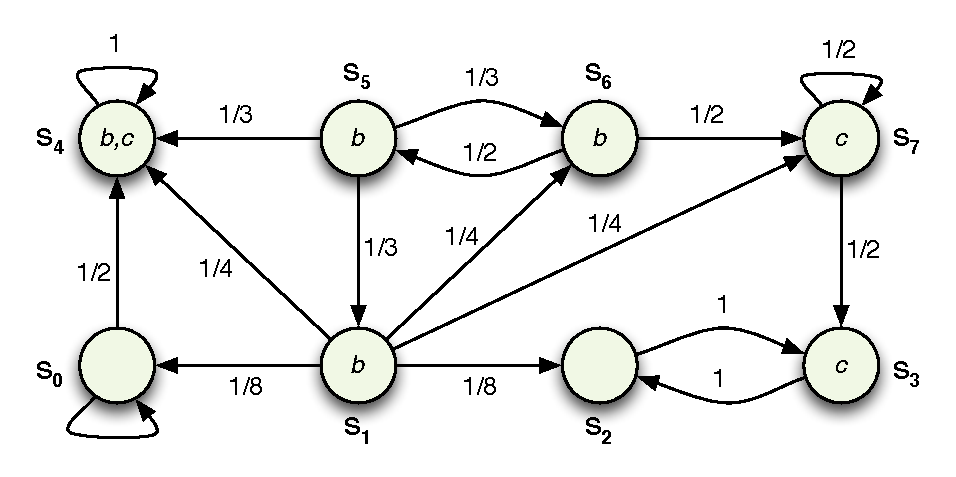
\includegraphics[scale=.85]{../GFX/ExerciseFigure3.pdf}
	\end{center}
	\caption{DTMC for question A2.4}
	\label{fig:2a4}
\end{figure}

We have to consider the DTMC in Figure \ref{fig:2a4}, which we will call $\mathcal{M} = \left(S, \mathbf{P}, s_1, AP, L\right)$, where $AP = \{b,c\}$. The initial state is $s_1$ and the labels are shown on the states.

\subsubsection*{2A.4a) Determine which states satisfy $\mathbb{P}_{\geq\frac{17}{19}}(b\;U\;c)$}
The set of satisfying states is:
$$\{s_3, s_4, s_6, s_7\}$$

\subsubsection*{2A.4b) Determine which states satisfy $\mathbb{P}_{\geq\frac{1}{2}}\left(X\;\mathbb{P}_{>\frac{1}{3}}\left( \left(b \vee c \right) U^{\leq 2} \left( b \wedge c \right) \right) \right)$}
The set of satisfying states is:
$$\{s_0, s_4, s_6\}$$

\chapter*{Part B: Intermediate Problems}
\section*{B1) Practical Problems}

\section*{B2) Theoretical Problems}
\subsection*{B2.1}
A step bounded formula $\Phi_1\;U^{\leqslant n}\;\Phi_2$ satisfies the needs for making assumptions regarding a specific type of interval, $I = [0, n]$, we would like to introduce a more generalized operator in the form of:
$$\Phi_1\;U^{I}\;\Phi_2 \quad | \quad I \in \left\{\;[n,n'],\;[n, n'[,\;]n, n],\;]n, n'[\;\right\} \quad | \quad 0 \leq x \leq y$$

\subsubsection*{B2.1a)}
To make this new operator possible using only PCTL, we have to synthesize the new operator using our currently available operators. We're not allowed to simply modify the current until operator to satisfy more cases, such a modification could be like:
$$\Phi_1\;U^{[n, \infty[}\;\Phi_2 = \Phi_1\;U^{\geqslant n}\;\Phi_2$$
Which would state that after $n$ steps $\Phi_1$ should hold up until at some point where $\Phi_2$ would hold.\\
\\
There are 10 important cases of how the intervals can be constructed, let's look at them case by case:
\begin{description}
	\item[Case 1:] $[0, 0]$\\
	This is the same as skipping the left part of the operator:
	$$\Phi_2$$

	\item[Case 2:] $[0, n]$\\
	This is the same as the current bounded until operator:
	$$\Phi_1\;U^{\leqslant n}\;\Phi_2$$
	
	\item[Case 3:] $[0,n[$ where $0 < n$\\
	This is the same as an interval of $[0, n-1]$, therefore it will either match \textbf{Case 1} or \textbf{Case 2}.
	
	\item[Case 4:] $[0, \infty[$\\
	This is the same as the unbounded until operator, so we would write this as:
	$$\Phi_1\;U\;\Phi_2$$
	
	\item[Case 5:] $[n, \infty[$\\
	Not possible as you would have to set a restriction of when the left part of the operator should apply. If we were to have a \emph{Time Step} operator, this would be possible.\\
	Let's define a time step operator, first we need a symbol for it:
	$$\mathbb{T}$$
	Then we need a syntax:
	$$\mathbb{T}^{\leqslant n} = \left\{
		\begin{array}{c l}
			\text{true} & \text{if } n \leq \text{amount of time steps passed}\\
			\text{false} & \text{if } n > \text{amount of time steps passed}
		\end{array}
	\right.$$
	$$\mathbb{T}^{\geqslant n} = \left\{
		\begin{array}{c l}
			\text{true} & \text{if } n \geq \text{amount of time steps passed}\\
			\text{false} & \text{if } n < \text{amount of time steps passed}
		\end{array}
	\right.$$
	Formally the syntax states that if the expression for $n$ satisfies for the amount of time steps passed then it returns \textbf{true}, otherwise it will return \textbf{false}.\\
	\\
	We can use this new operator to specify a starting point for our modified until operator. Using the new syntax we can properly write out the adapted PCTL for the case:
	$$\mathbb{T}^{\geqslant n} \wedge \mathbb{P}_{=1}\left(\Phi_1\;U\;\Phi_2\right)$$
	
	\item[Case 6:] $]0, \infty[$\\
	This can be rewritten to $[1, \infty[$, which can be interpreted as $[n, \infty[$. See Case 5.
	
	\item[Case 7:] $]n, \infty[$ where $0 < n$\\
	This can be rewritten to $[n+1, \infty[$, which is covered by Case 5.
	
	\item[Case 8:] $[n, n']$\\
	We have to make use of our \emph{Time Step} operator again. This time there's both a limitation of when to start and a limitation of when to end.
	$$\mathbb{T}^{\geqslant n} \wedge \mathbb{P}_{=1}\left(\Phi_1\;U^{\leqslant n'}\;\Phi_2\right)$$
	
	\item[Case 9:] $]n, n']$ where $n < n'$\\
	This can be rewritten to $[n+1, n']$
	
	\item[Case 10:] $]n, n'[$ where $n < n + 1 < n'$\\
	This can be rewritten to $[n+1, n'-1]$.
\end{description}

\subsubsection*{B2.1b)}
\subsubsection*{B2.1c)}
\subsubsection*{B2.1d)}

\subsection*{B2.2}
\begin{figure}[H]
	\begin{center}
		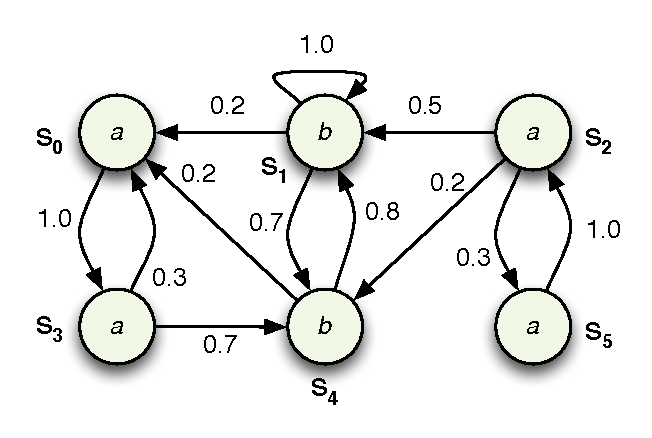
\includegraphics[scale=.85]{../GFX/ExerciseFigure4.pdf}
	\end{center}
	\caption{DTMC for question B2.2}
	\ref{fig:b22}
\end{figure}

\subsubsection*{B2.2a)}
\subsubsection*{B2.2b)}
\subsubsection*{B2.2c)}
\subsubsection*{B2.2d)}
\subsubsection*{B2.2e)}
\subsubsection*{B2.2f)}

\chapter*{Part C: Advanced Problems}
\section*{Practical Problems}

\end{document}
